\chapter{Process Models}
\label{github}


This section contains larger images of the process models compared to the versions inside the text. Alternatively, they are also uploaded to GitHub.

The GitHub Repository contains the diagrams in both their original source format and in high-resolution image format. It also includes the origiginal Latex-files to compile the final version of this project paper.

The repository is available to public at:

\noindent\url{https://github.com/wuestm/saps}



\begin{figure}[h]
    \centering
    \includegraphics[width=1.0\linewidth, angle=90, origin=c]{images/bpmn/Wizard_all_flows.pdf} 
    \caption{Wizard Data complete Control Flow Model}
    \label{fig:wizard_flow_all_paths}
\end{figure}

\begin{figure}
    \centering
    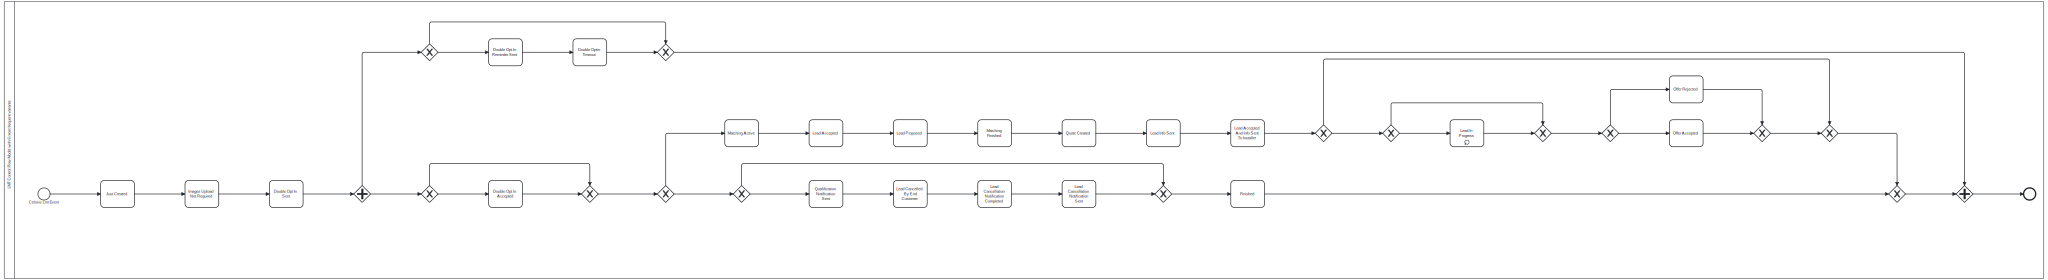
\includegraphics[width=1.0\linewidth, angle=90, origin=c]{images/bpmn/LMT_5_Variants.pdf}
    \caption{LMT Data Control Flow Model with 5 most frequent variants}
    \label{fig:appendix_LMT_5_variants}
\end{figure}

\begin{figure}
    \centering
    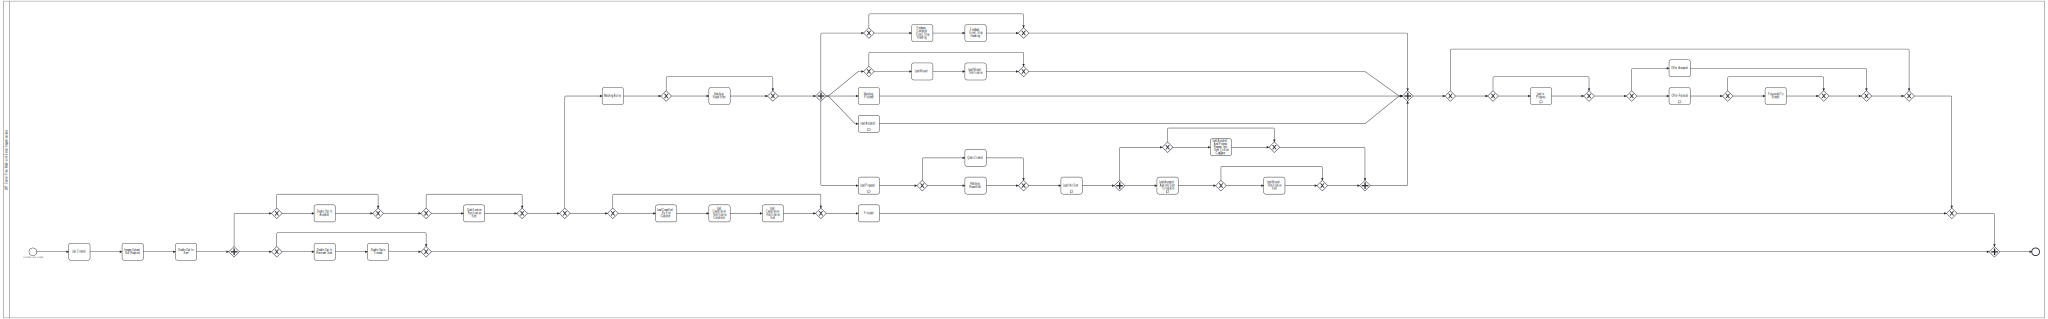
\includegraphics[width=1.0\linewidth, angle=90, origin=c]{images/bpmn/LMT_8_Variants.pdf}
    \caption{LMT Data Control Flow Model with 8 most frequent variants}
    \label{fig:appendix_LMT_5_variants}
\end{figure}

\begin{figure}
    \centering
    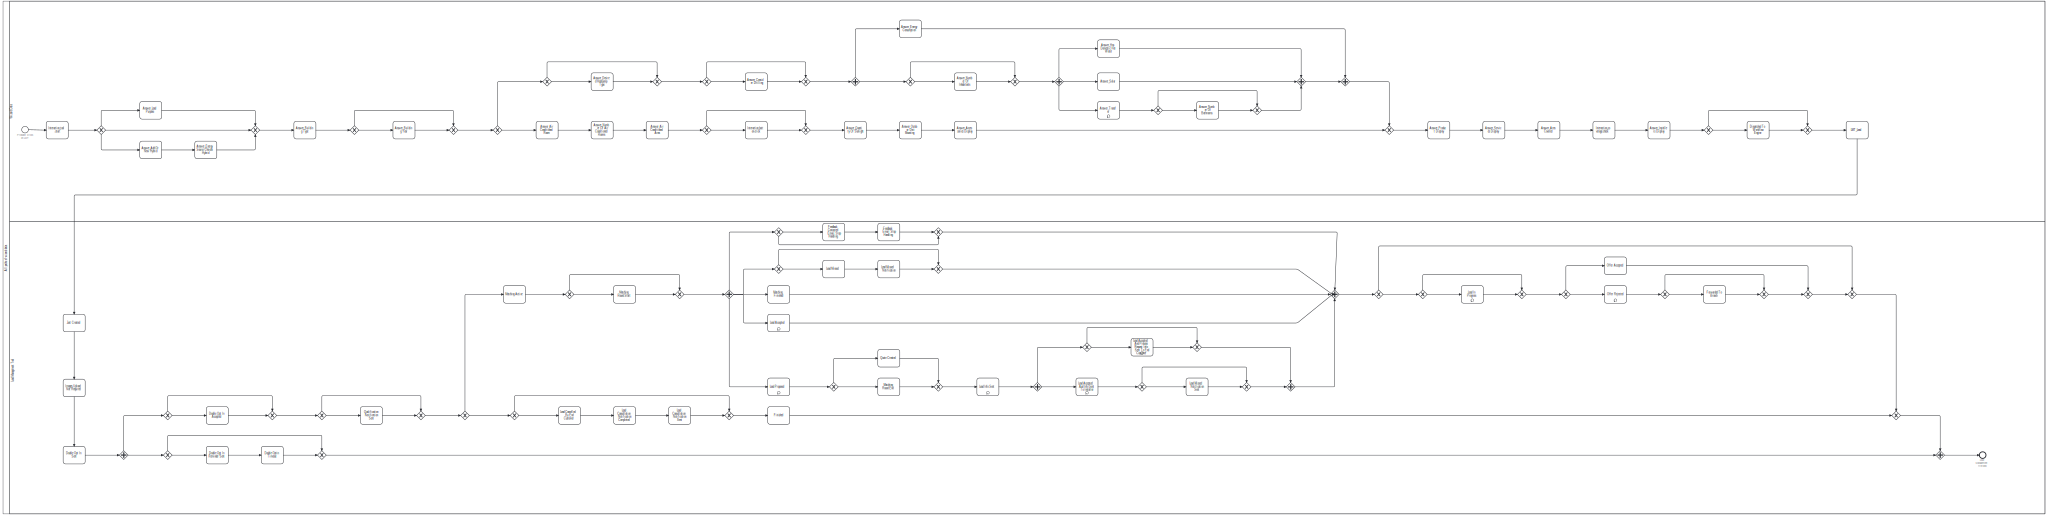
\includegraphics[width=1.3\linewidth, angle=90, origin=c]{images/bpmn/Wizard_LMT_combined_V2.pdf}
    \caption{Wizard and LMT combined Control Flow Model}
    \label{fig:wizard_lmt_combined}
\end{figure}